\documentclass[letterpaper,12pt]{article}

\setlength{\topmargin}{0in}
\setlength{\textheight}{9.0in}
\setlength{\textwidth}{6.5in}
\setlength{\columnsep}{0.25in}
\setlength{\headheight}{0in}
\setlength{\headsep}{0in}
\setlength{\oddsidemargin}{0.0in}
\setlength{\evensidemargin}{0.0in}
\setlength{\topskip}{0in}
\usepackage{times}
\usepackage{mdwlist}
\usepackage{hyperref}
\usepackage{array}
\usepackage{multicol}
\usepackage{enumitem}
\usepackage{graphicx}
\usepackage{amsmath}
\usepackage{lipsum}
\hypersetup{colorlinks=true}
\renewcommand{\baselinestretch}{1.00}

\newcounter{exanum}
\setcounter{exanum}{1}
\newcommand{\exercise}{\subsubsection*{Exercise \#\theexanum: \refstepcounter{exanum}}}

\newcommand{\duedate}{end of day, October 03, 2030}

\newcommand{\courseyear}{Fall 2019}
\newcommand{\system}{Stampede2}

\input{vc}


\begin{document}
\begin{flushright}
\VCDateISO \\
Rev: \VCRevision
\end{flushright}

\vspace*{0.05cm}
\subsection*{Tools and Techniques for Computational Science - \courseyear{}}
\vspace*{-.2cm}
\noindent{{\large \em Assignment Latex Example}

\vspace*{15pt}

\subsection*{Shell Scripts, Batch Jobs}

Please answer the following questions and commit your resulting
scripts to your assigned GitHub repository.
(https://github.com/uthpc/student-{\em yourgithubId}.git).  You should
commit periodically while working on the shell scripts and have a
minimum of 5 commits per script (with relevant commit
messages). \\

\noindent {\em Note}: scripts requiring command-line arguments to run should print the
script's intended usage and exit with an error if the minimum number
of arguments is not provided.

\noindent\rule{\textwidth}{0.4pt} \\

\exercise

(25 pts) Do something awesome. \\

\noindent \lipsum[1]
\vspace*{20pt}

\exercise

(25 pts) Do something clever. \\

\noindent \lipsum[2]


\clearpage
\exercise

(50 pts) Combine your awesomeness and cleverness.

\begin{figure}[h]
\begin{center}
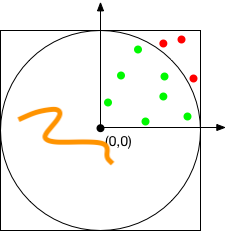
\includegraphics[width=2.2in]{pi-circle.png}
\end{center}
\vspace*{-.7cm}
\caption{Circle of radius 0.5 enclosed by a 1x1 square.
 -}
\label{fig:circle}
\end{figure}

\noindent \lipsum[2-3]


\end{document}
